\documentclass[11pt,a4paper]{article}

% ------ PACKAGES ------

\usepackage[utf8]{inputenc}%encodage en utf8
\usepackage[english]{babel} %permet caractères français
\usepackage[T1]{fontenc} %permet cararct spéciaux
\usepackage{hyperref}  %liens hypertextes

\usepackage{array}
\usepackage{float}
\usepackage{lscape}

\usepackage{amsmath,amsthm} %pour les maths
\usepackage{commath}
\usepackage{setspace}%pour avoir un inteligne de 1.5

\usepackage{multirow}  %Tableaux à plusieurs lignes

\usepackage{geometry}%réglages mise en page
\usepackage{fancyhdr}%for headers and footers

\usepackage{algorithm}
\usepackage{algorithmic}
\usepackage{optidef} %formules d'optimisation
\usepackage{subcaption}
\usepackage{parskip}

\newtheorem{theorem}{Theorem}
\newtheorem{defn}[theorem]{Definition}
\newtheorem{example}[theorem]{Example}
\newtheorem{remark}[theorem]{Remark}
\newtheorem{question}[theorem]{Question}

\newtheorem{lemma}[theorem]{Lemma}
\newtheorem{claim}[theorem]{Claim}
\newtheorem{prop}[theorem]{Proposition}
\newtheorem{corollary}[theorem]{Corollary}
\newtheorem{conjecture}[theorem]{Conjecture}

\newtheorem{hyp}[theorem]{Hypothesis}

\onehalfspacing   %interligne de 1.5

\renewcommand{\algorithmicrequire}{\textbf{Input:}}
\renewcommand{\algorithmicensure}{\textbf{Output:}}

% ------ ADD SUBSUBSECITONS ------
\setcounter{secnumdepth}{5}

% ------ PAGE LAYOUT ------
\geometry{
%a4paper
%body={170mm,260mm},
left=35mm, top=25mm,
bottom=25mm, right=25mm
%headheight=10mm, headsep=10mm,
%footskip=10mm
}

% ---------- COMMAND SETTERS -----------

\newcommand{\HRule}{\rule{\linewidth}{0.5mm}} %newcommand for cover page

\begin{document}
\begin{titlepage}
\begin{center}

\textsc{\LARGE universit\'e libre de bruxelles}\\[2.5cm]

% Upper part of the page. The '~' is needed because \\
% only works if a paragraph has started.

\includegraphics[width=0.3\textwidth]{Images/ulblogo.jpg}~\\[1cm]

\textsc{\Large  TRAN-F501 \\[0.3cm] Internship - 201819 }\\[0.5cm]

% Title
\HRule \\[0.6cm]
{ \huge \bfseries Project:
A stochastic simulation system for protein aggregation \\[0.6cm] }

\HRule \\[2cm]

% Author and supervisor

\begin{center} \large
\emph{Supervisor:} \\
Tom \textsc{Lenaerts}\\


\emph{Author:}\\
Prateeba\textsc{ Ruggoo}\\
\end{center}

\vfill

% Bottom of the page
{\large \today}

\end{center}
\end{titlepage}


\tableofcontents \pagebreak

\section{Introduction}
Diseases like Alzheimer and Parkinson disease are the result of proteins aggregating into large fractal structures that hinder the cell function or even destroy them. Understanding how aggregates are formed and change over time is important to understand when they become harmful and how maybe treatments affect aggregate formation.

The goal of this Internship is to implement a simulation system to study aggregation between proteins and  is performed in collaboration with the Switch lab in the KU Leuven, who has an extensive expertise in studying aggregation and related diseases.

\subsection{Mathematical modeling}
The principle task is to develop a method for simulating the time evolution of the $N$ quantities $\{X_{i}\}$, knowing only their initial values $\{X_{i}^{(0)}\}$, the form of the $M$ reactions $\{R_{\mu}\}$ and the values of the reaction parameters $\{c_{\mu}\}$.
There are two fundamental approaches to the mathematical modelling of chemical reactions.
\begin{enumerate}
  \item Deterministic models which are based on differential equations.
  \item Stochastic simulations where the fundametal principle is that molecular reactions are essentially random processes i.e it is impossible to say with complete certainty the time at which the next reaction will occur. This approach uses basic Newtonian physics and thermodynamics to arrive at a form defined as the propensity function that gives the probability $a_\mu$ of reaction $\mu$ occuring in time interval ($t, t+\delta t$).
\end{enumerate}

\section{Gillespie's stochastic framework of chemical kinetics}
\begin{defn}{Problem definition:}
We are given a volume $V$ containing molecules of $N$ chemically active species $S_{i}(i = 1, \dots, N)$. Let $X_{i} \equiv$ current number of molecules of chemical species $S_{i} \in V, (i = 1, 2, \dots, N)$ and let $R_{\mu} (\mu = 1, \dots, M)$ be the chemical reactions in which the species $S_{i}$ can participate. Each reaction $R_{\mu}$ is characterized by a numerical reaction parameter $c_{\mu}$. The goal is to simulate the trajectories of the $N$ chemically active species $S_i$ and predict which reaction will occur at each time step according to the correct probability distribution.
\end{defn}

\begin{defn}{}
The reaction parameter $c_{\mu}$ is defined so that $c_{\mu} \delta t$ gives the probability that a randomly chosen molecule of chemical species $S$ reacts during the time interval [$t, t+ \delta t$] where $t$ is time and $\delta t$ is an infinitesimally small time step.
\end{defn}

\begin{defn}{}
The probability that exactly one reaction $\mu$ occurs during the infinitesimal time interval [$t, t+ \delta t$] is equal to $S(t)k \delta t$ where $S(t)$ is the number of chemical species $S$ at time $t$.
\end{defn}

\begin{defn}{}
State of the system is defined by the number of molecules of each species and changes discretely whenever one of the reactions is executed.
\end{defn}

\subsection{Gillespie's Direct Method}
Given the problem defined above, the Gillespie's Direct Method answers two questions :
\begin{enumerate}
  \item Which reaction occurs next ?
  \item When does it occur ?
\end{enumerate}

  \subsubsection{Gillespie's Direct Method formulas}
  \begin{enumerate}
    \item Probability density $P(\mu, \tau)$ that the next reaction is $\mu$ and that it occurs at time $\tau$ is given by : \\ $P(\mu, \tau)d\tau = a_{\mu}exp(-\tau \sum_{j}a_{j})d\tau$. \label{itm:(eq 1)}
    \item Probability that the next reaction is reaction $\mu$ is given by : \\  $Pr(Reaction = \mu) = a_{\mu} / \sum_{j}a_{j}$. \label{itm:(eq 2)}
    \item Probability distribution for times \\  $P(\tau)d\tau = (\sum_{j}a_{j})exp(-\tau \sum_{j}a_{j})d\tau$.\label{itm:(eq 3)}
  \end{enumerate}

\subsubsection{Gillespie's Direct Method : Pseudo code}
\begin{algorithm}[!h]                     % enter the algorithm environment
\caption{Gillespie's Direct Method}       % give the algorithm a caption
\begin{algorithmic}                       % enter the algorithmic environment
\REQUIRE $N$ chemically active species $S_i, \{X_{i}^{(0)}\}$ initial values of each species $S_i$, the set $R$ \hspace*{8mm} of chemical reactions and the reaction parameter $c_{\mu}$ for each reaction.
\ENSURE Sample trajectory of a chemical process in the stochastic framework.
\WHILE{!$($simulation time exceeded$)$ }
    \STATE 1. Initialization: Set initial number of molecules in the system, set $t \leftarrow 0$.
    \STATE 2. Calculate the propensity function, $a_{i},  \forall i$.
    \STATE 3. Choose $\mu$ according to the distribution in \ref{itm:(eq 2)}.
    \STATE 4. Choose $\tau$ according to an exponential with parameter $\sum_{j}a_{j}$ as in \ref{itm:(eq 3)}.
    \STATE 5. Update the number of molecules to reflect execution of reaction $\mu$. Set $t \leftarrow t + \tau$.
    \STATE 6. Go to step 2.
\ENDWHILE
\end{algorithmic}
\label{alg:Gillespie's Direct Method}
\end{algorithm}

\subsubsection{Gillespie's Direct Method : Example}
The source code of the Direct method simulation model can be found at \href{https://github.com/Prateeba/TRAN-F501-Internship-201819/tree/master/Code/G_first_reaction}{Direct-method-github}. The reaction set is the example used in Gillespie's paper \cite{gillespie_general_1976}.
\begin{gather}
  {X \xrightarrow{c_{1}} Y}      \\
  {Y \xrightarrow{c_{2}} X}      \\
  {2X \xrightarrow{c_{3}} Z}     \\
  {Z \xrightarrow{c_{4}} 2X}     \\
  {W + X \xrightarrow{c_{5}} 2X} \\
  {2X \xrightarrow{c_{6}} W + X}
\end{gather}
where the reaction parameters $c_{i} \in (i = 1, 2, \dots, 6)$ is equal to [1,1,2,1,2,1] respectively and the initial number of each species is $= 10$.
\begin{example}{Generating a sample trajectories of a chemical process in the stochastic framework : Direct Method}
    \begin{figure}[!h]
    \centering
    \begin{subfigure}{.5\textwidth}
      \centering
        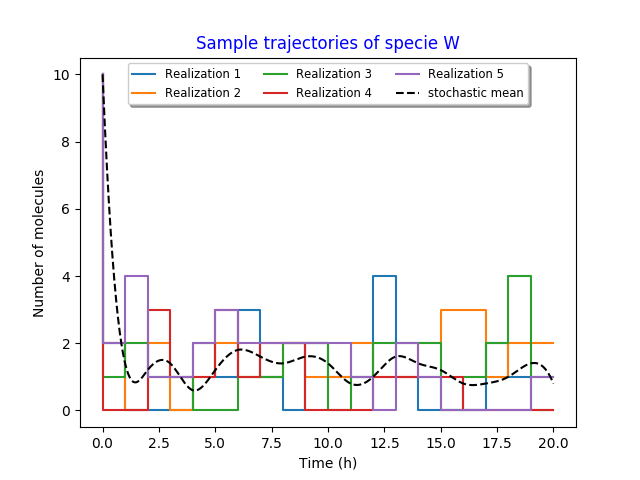
\includegraphics[width=1.1\linewidth]{Images/w_5.png}
        \label{fig: Single sample trajectory}
    \end{subfigure}%
    \begin{subfigure}{.5\textwidth}
      \centering
        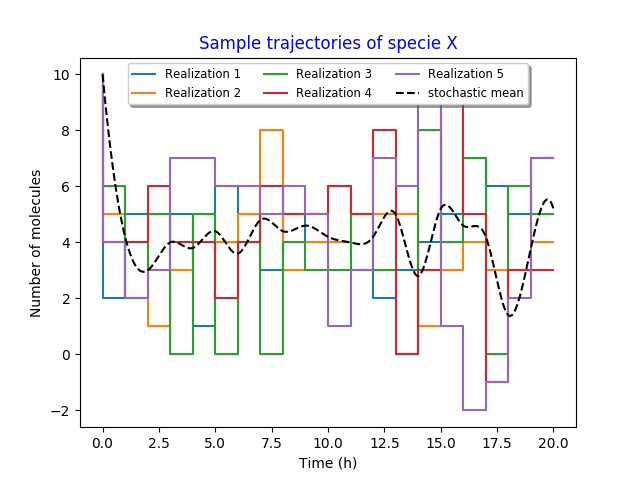
\includegraphics[width=1.1\linewidth]{Images/x_5.png}
        \label{fig: Single sample trajectory}
    \end{subfigure}
    \centering
    \begin{subfigure}{.5\textwidth}
      \centering
        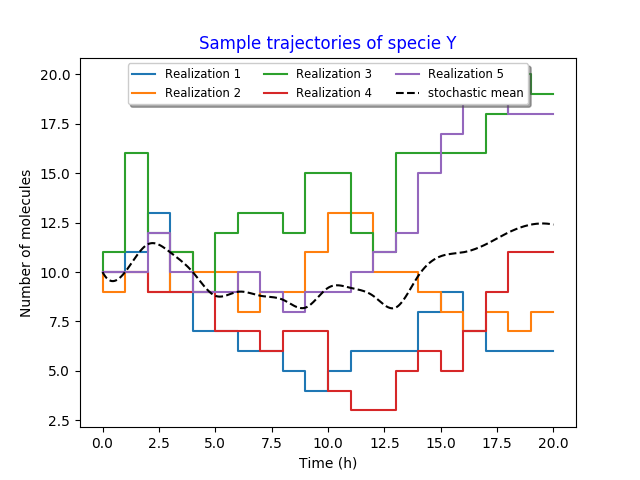
\includegraphics[width=1.1\linewidth]{Images/y_5.png}
        \label{fig: Single sample trajectory}
    \end{subfigure}%
    \begin{subfigure}{.5\textwidth}
      \centering
        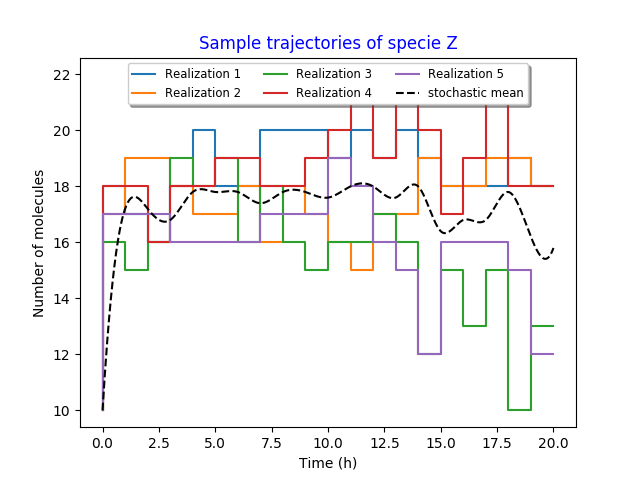
\includegraphics[width=1.1\linewidth]{Images/z_5.png}
        \label{fig: Single sample trajectory}
    \end{subfigure}
    \caption{The x-axis denotes the duration time of the simulation and the y-axis denotes the number of molecules of each species $S_{i}$ at each time step.}
    \end{figure}
\end{example}

\subsection{Gillespie's Next Reaction Method}
The goal of the next reaction method is to do away with the above processes and update only data that has been modified. The main idea is to generate a putative time $\tau_i$ for each reaction $i$ that will occur and choose the reaction $\mu$ whose putative time $\tau_{\mu}$ is least. In order to minimize the computation time, the Next Reaction Method is implemented using specific data structures.
To make the sampling of reactions more efficient, an indexed priority queue is used to store the reaction times. On the other hand, to make the recomputation of propensities more efficient, a dependency graph is used. This dependency graph tells which reaction propensities to update after a particular reaction has fired.

\subsubsection{Gillespie's Next Reaction Method : Pseudo code} \ref{alg:Gillespie's Next Reaction Method}
\begin{algorithm}[!h]                            % enter the algorithm environment
\caption{Gillespie's Next Reaction Method}       % give the algorithm a caption
\begin{algorithmic}                              % enter the algorithmic environment
\REQUIRE $N$ chemically active species $S_i, \{X_{i}^{(0)}\}$ initial values of each species $S_i$, the set $R$ of \hspace*{8mm} chemical reactions and the reaction parameter $c_{\mu}$ for each reaction.
\ENSURE Sample trajectory of a chemical process in the stochastic framework.
\WHILE{!$($simulation time exceeded$)$ }
    \STATE 1. Initialization :
      \STATE \ \ \ 1.1  \ set initial number of molecules, set $t \leftarrow 0$, generate a dependency graph $G$.
      \STATE \ \ \ 1.2. calculate the propensity function, $a_{i} ,  \forall i$.
      \STATE \ \ \ 1.3. for each $i$, generate a putative time, $\tau_{i}$, according to an exponential
      \STATE \ \ \ \ \ \ \ \ \ distribution with parameter $a_{i}$.
      \STATE \ \ \ 1.4. store the $\tau_{i}$ values in an indexed priority queue $P.$
    \STATE 2. Let $\mu$ be the reaction whose putative time, $\tau_{\mu}$, is least.
    \STATE 3. Let $\tau$ be $\tau_{\mu}$.
    \STATE 4. Update the number of molecules to reflect execution of reaction $\mu$. Set $t \leftarrow \tau$.
    \STATE 5. For each edge($\mu$, $\alpha$) in the dependency graph $G$,
    \STATE \ \ \ 5.1 update $a_{\alpha}.$
    \STATE \ \ \ 5.2 if $\alpha \neq \mu$, set $\tau_{alpha} \leftarrow (a_{\alpha,old}/a_{\alpha, new})(\tau_{\alpha} - t) + t.$
    \STATE \ \ \ 5.3 if $\alpha = \mu$, generate a random number, $\rho$, according to an exponential distribution \hspace*{8mm} with parameter $a_{\mu}$ and set $\tau_{\alpha} \leftarrow \tau + t.$
    \STATE \ \ \ 5.4 Update the old $\tau_{\alpha}$ value in $P$.
    \STATE 6. Go to step $2$.
\ENDWHILE
\end{algorithmic}
\label{alg:Gillespie's Next Reaction Method}
\end{algorithm}

\subsubsection{Gillespie's Next Reaction Method : Example}
The source code Next Reaction Method can be found at \href{https://github.com/Prateeba/TRAN-F501-Internship-201819/tree/master/Code/G_next_reaction}{Next-Reaction-Method-github}. The reaction set is the example used in the following paper \cite{gibson_efficient_2000}.
\begin{gather}
  {A + B \xrightarrow{k_{1}} C}      \\
  {B + C \xrightarrow{k_{2}} D}      \\
  {D + E \xrightarrow{k_{3}} E + F}     \\
  {F \xrightarrow{k_{4}} D + G}     \\
  {E + G \xrightarrow{k_{5}} A} \\
\end{gather}
where the reaction parameters $k_{\mu} \in (i = 1, 2, \dots, 5)$ is equal to [1,2,2,2,1] respectively and the initial number of each species is $= 10$.
\begin{example}{Generating a sample trajectories of a chemical process in the stochastic framework : Next Reaction Method}
    \begin{figure}[H]
    \centering
    \begin{subfigure}{.5\textwidth}
      \centering
        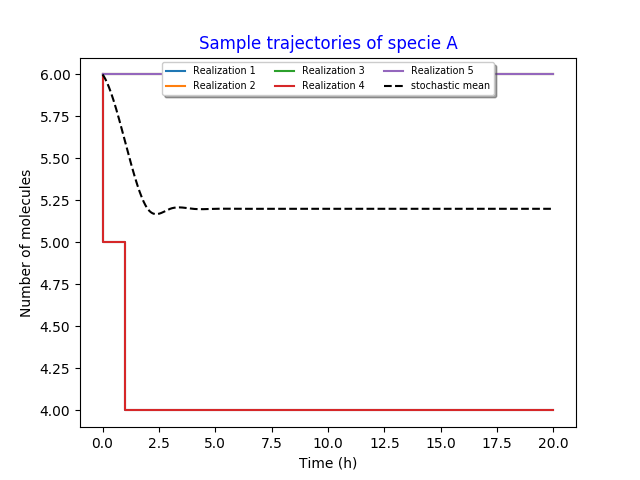
\includegraphics[width=1.1\linewidth]{Images/a.png}
        \label{fig: Single sample trajectory}
    \end{subfigure}%
    \begin{subfigure}{.5\textwidth}
      \centering
        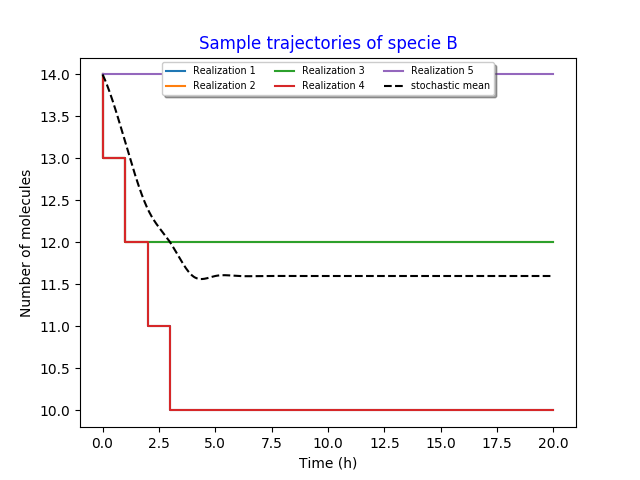
\includegraphics[width=1.1\linewidth]{Images/b.png}
        \label{fig: Single sample trajectory}
    \end{subfigure}
    \centering
    \begin{subfigure}{.5\textwidth}
      \centering
        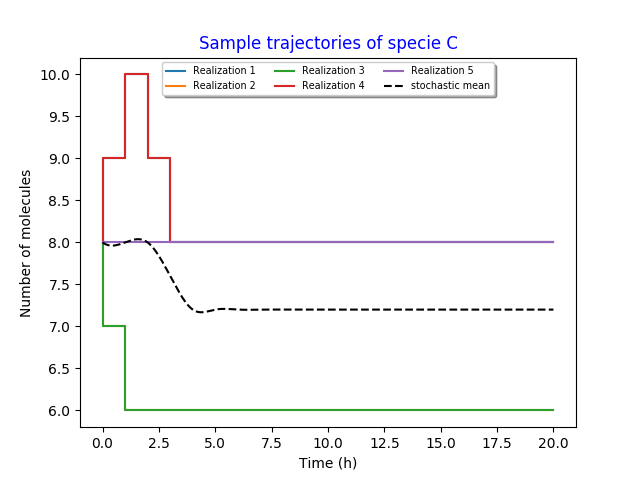
\includegraphics[width=1.1\linewidth]{Images/c.png}
        \label{fig: Single sample trajectory}
    \end{subfigure}%
    \begin{subfigure}{.5\textwidth}
      \centering
        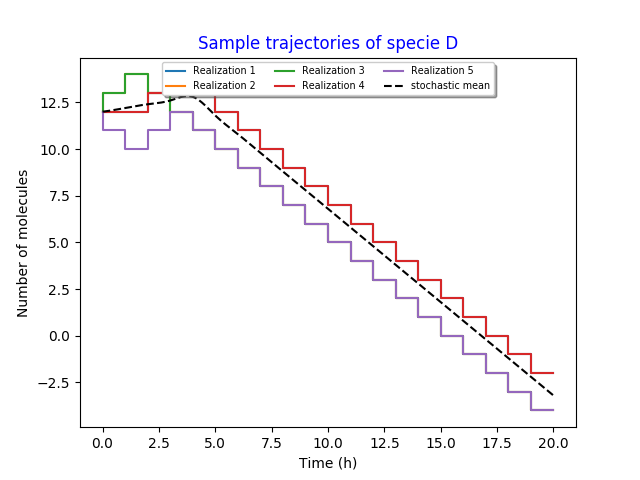
\includegraphics[width=1.1\linewidth]{Images/d.png}
        \label{fig: Single sample trajectory}
    \end{subfigure}
    \centering
    \begin{subfigure}{.5\textwidth}
      \centering
        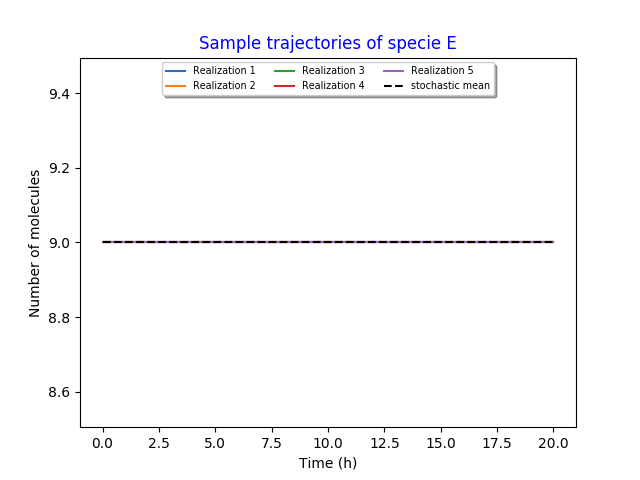
\includegraphics[width=1.1\linewidth]{Images/e.png}
        \label{fig: Single sample trajectory}
    \end{subfigure}%
    \begin{subfigure}{.5\textwidth}
      \centering
        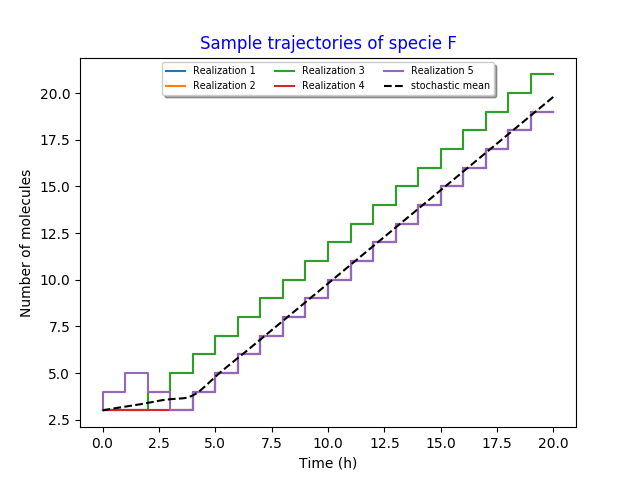
\includegraphics[width=1.1\linewidth]{Images/f.png}
        \label{fig: Single sample trajectory}
    \end{subfigure}
    \centering
    \begin{subfigure}{.5\textwidth}
      \centering
        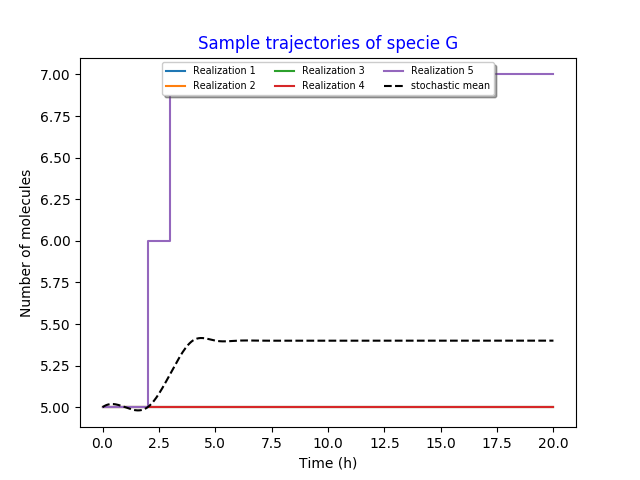
\includegraphics[width=1.1\linewidth]{Images/g.png}
        \label{fig: Single sample trajectory}
    \end{subfigure}%
    \caption{The x-axis denotes the duration time of the simulation and the y-axis denotes the number of molecules of each species $S_{i}$ at each time step.}
    \end{figure}
\end{example}

\section {Molecular mechanisms of protein aggregation}
Until now, all what was done is using random reaction parameters for each reaction in the stochastic simulation. However in order to study the protein aggregation, understanding the kinetics of the aggregation is fundametal. In the following paper \cite{meisl_molecular_2016}, a protocol is described on how to make full use of kinetic descriptions derived from a model of the underlying microscopic reactions that make up the aggregation network. The fitted parameters are therefore meaningful and correspond to physical properties of the system, such as nucleus sizes, rate constants of individual reactions and saturation concentrations.

The key idea is to analyze a large data set of multiple kinetic traces at different reagent concentrations simultaneously,with a single rate law and yield strong mechanistic constraints that will be helful in choosing the appropriate models.

\subsection{Obtaining qualitative constraints : Half times}
Given a dataset, several fundametal models can be considered for the fitting process to yield the rate constants. In order to choose the best model, adding some constraints based on the concentration dependence of the aggregation reaction is a solution. A helpful qualitative constraint is half times.
\begin{defn}{} Half-time is defined as the time at which the signal has reached half of its final plateau value. \end{defn}
Normalised data and the monomer concentration of each repeat is used for this process. By plotting Log(half time) versus Log(monomer concentration) plot, the slope known as the scaling exponent gives insight as to which about the dominant process of fibre multiplication, which in turn can be used to decide on possible models for the fitting. By considering how the half times scale with monomer concentration and how this scaling depends on the monomer concentration, one can obtain constraints on possible mechanisms.

Very generally, a negative curvature in the double logarithmic plots (i.e., when the slope becomes steeper at higher
monomer concentrations, and therefore the process more monomer dependent) is indicative of competition between several
processes in parallel. A positive curvature, in contrast (i.e., a flattening of the curve at higher monomer concentrations, and thus
a decrease in monomer dependence), suggests the presence of a saturation effect in a serial process  or, in rare cases, at monomer concentrations close to solubility, it can be due to a change in nucleus size9. The behavior of half-times with varying monomer concentration is, therefore, a
good first guide to narrowing down the number of possible models, because it limits the number of acceptable reaction networks
by determining the reaction order of the dominant process and probing for competition or saturation effects. The model for fitting needs to be chosen to reflect these findings.

\subsubsection{Log(half time) versus Log(monomer concentration) plot}
\begin{example}{To set title}
  \begin{figure}[H]
  \centering
  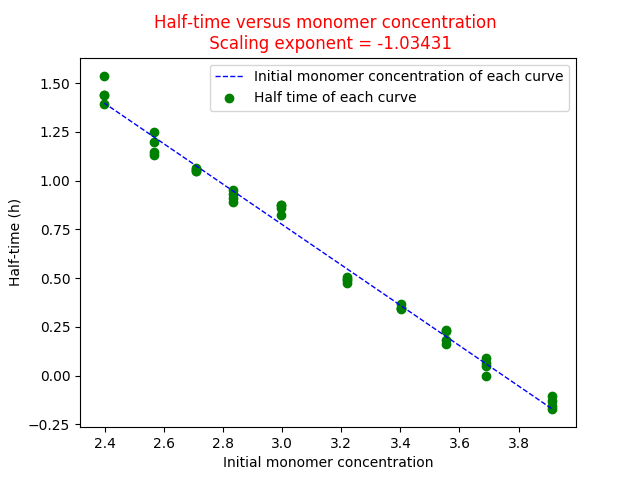
\includegraphics[width=1\textwidth]{Images/half_time_vs_monomer.png}
  \caption{The x-axis denotes the time used and the y-axis denotes the number of molecules : Sample 2}
  \label{fig: sample trajectory}
  \end{figure}
\end{example}
The source code to generate the log off plot of a given dataset can be found at \href{https://github.com/Prateeba/TRAN-F501-Internship-201819/tree/master/Code/Fitting}{Next-Reaction-Method-github}.


\subsection{From Half-times to models}
\begin{figure}[H]
\centering
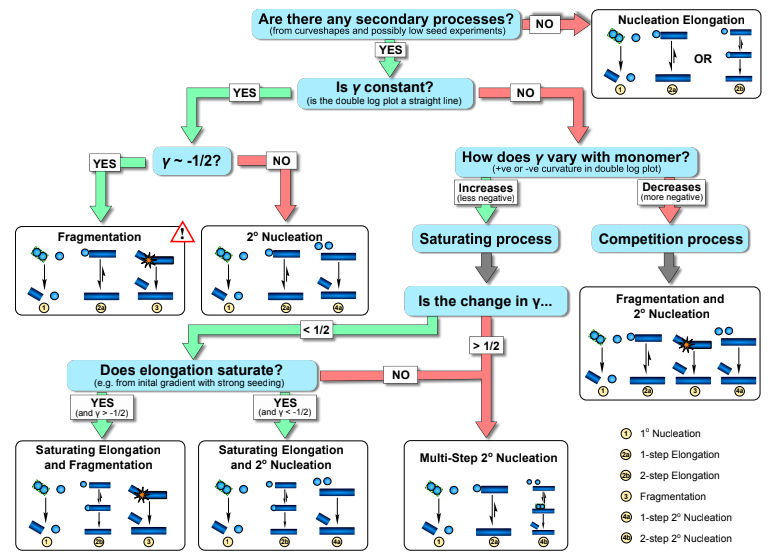
\includegraphics[width=1\textwidth]{Images/half_times_to_models.png}
\caption{The curvature of the double logarithmic plots and the value of their slopes gives insights into which aggregation mechanisms are dominant. The flowchart illustrates the decision process to arrive at a likely model, based on the half time plots.}
\label{fig: sample trajectory}.
\end{figure}




\section{Results}
\subsection {Amylofit's parameters estimation}

\subsection{My program's parameter estimation}

\subsection{Amylofit's estimated parameters in Gillespie stochastic framework}

\subsection{My estimated parameters in Gillespie stochastic framework}


\section{Conclusion}






\clearpage
\bibliographystyle{alpha}
\bibliography{combinatorial}


\end{document}
